\documentclass[tikz,border=10pt]{standalone}
\begin{document}

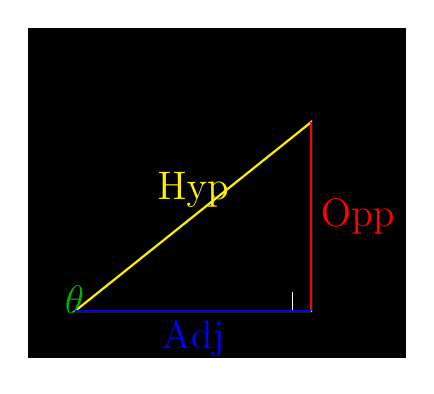
\begin{tikzpicture}[scale=3]

    % Background color
    \fill[black] (-0.2,-0.2) rectangle (1.4,1.2);

    % Triangle
    \draw[thick, yellow] (0,0) -- (1,0) -- (1,0.8) -- cycle;
    
    % Right angle marker
    \draw[white] (1,0) -- ++(-0.08,0) -- ++(0,0.08);

    % Labels
    \node[left, green!70!black] at (0.08,0.05) {\Large $\theta$};
    \node[above, yellow] at (0.5,0.4) {\Large Hyp};
    \node[right, red] at (1,0.4) {\Large Opp};
    \node[below, blue] at (0.5,0) {\Large Adj};

    % Side colors
    \draw[thick, red] (1,0) -- (1,0.8);
    \draw[thick, blue] (0,0) -- (1,0);

\end{tikzpicture}

\end{document}
